% !TeX spellcheck = en_GB

The Least Cost Path algorithm is used to plan a possible route for a power line.
The Least Cost Path algorithm is a Dijkstra algorithm~\cite{dijkstra_note_1959} applied on a raster map.
The vertices of the graph are the pixel centres, that are connected to the eight neighbouring pixel centres via the edges.
This makes it possible to find routes on graphs that are not predefined, such as road networks.
The weights of the edges are the local costs of transit from one pixel center to the neighbouring pixel center.
The costs can be physical costs, such as the local slope, but also can be composed of other factors as the acceptance rate to transverse a given land usage.
The Least Cost Path algorithm consists of at least two successive steps.
1) The first step is to aggregate the costs of travelling from the starting point to a given set of end points.
This step generates the aggregated cost raster of travelling from the starting point to any point of the cost raster.
2) In the next step the backtracking, the route of the actual Least Cost Path is calculated.
For each end point the path via the lowest cost neighbour is taken until the starting point is reached.

Some implementations switch the roles of start and ending points, so that either many start points and one single end point, or one single end point and many end points can be used.
In some implementations there is an extra step between 1) and 2) that calculates cost-weight direction raster, that encodes the direction of the shortest
path to the starting point as integer values.

We retrieve a set of different spacial data-sets from  public sources as a basis for creating the cost raster.
The study area are the counties of Cuxhaven and Osterholz in the state of Lower Saxony, Germany.
Areas protected by different European and National conservation laws are provided by the German Environment Agency
as \acrfull{wfs}~\cite{noauthor_schutzgebiete_2015}.

The national land coverage (ATKIS) with a scale of 1:250000 are provided by the Federal Agency for Cartography
and Geodesy~\cite{noauthor_digitales_2021}.
The national power grid (tags: 'power': line) has been retrieved via OpenStreetMap~\cite{boeing_osmnx_2017}.
Local data as houses at Level of Detail 1 are provided by the State Office for Geoinformation and Land Surveying of
Lower Saxony~\cite{noauthor_opengeodatani_2022}.
In addition, local planning geodata for the land use are taken
from 'Metropolplaner' (Planning data Lower Saxony \& Bremen)~\cite{noauthor_metropolplaner_2022}.

PyWPS~\cite{noauthor_welcome_2016} is used to provide the Least Cost Path algorithm as a \acrfull{wps} in combination with flask~\cite{noauthor_flask_nodate}.
As client Birdy~\cite{noauthor_birdy_nodate} connects to the \acrshort{wps}, sends the cost raster and receives the resulting Least Cost Path.
The initial implementation of the Least Cost Path algorithm is based on the implementation for the QGIS-Plugin
'Least Cost Path'~\cite{noauthor_leastcostpathdijkstra_algorithmpy_2022} in version 1.0, but refactored to optionally export the aggregated costs.

In order to compute intermediate cost raster the different vector layers of the different entities are optionally filtered, buffered and then rasterised.
Filtering the layers of the vector files for special attributes enables further differentiation.
For example, it is possible to differentiate between heath and uncultivated land in the land cover.
Adding a buffer can be used either to convert a line object such as a power line and a road into a polygon (with the
correct physical width), or to add minimum distance from an existing of planed area to the new power line.
Each of theses intermediate rasters are given a weight (cost) which expresses the cost of using land covered by this layer.
In the final cost raster costs of all intermediate rasters are aggregated with the maximum function.
Thus, an area covered by several layers is uniformly associated with the highest cost.
Any place in the study area, that is not covered by any layer and thus does not yet have a weight, is given the default cost.

The costs have been grouped into five different levels~(see table~\ref{tab:1}), starting from \textit{Preferential} areas with
very low costs, via \textit{No restriction}s, which is the default, used when no other layers are covering the local area,
to \textit{Restricted}, \textit{Strongly Restricted} and \textit{Prohibited} areas with high costs.
These higher costs represent the degree to which a place with this cost should be avoided, while routing the path.
The ratio of the higher costs to the lower costs equals the detour
the algorithm is willing to go.
Thus, as \textit{prohibited} areas describe a legal obligation, not to use these areas or only to the utmost minimum,
the weight that resembles the costs for these types of areas is set especially high.\\

All these layers are provided as vectors.
The Least Cost Path algorithm uses raster data.
Rasterisation transforms a vector into a raster.
Rasterisation can be done in two different ways.
In both ways, the rasterisation can be imaged, as the old vector is superimposed on the new raster grid with the new
given resolution and the new affine transformation and the coordinate reference system of the vector.
Both rasterisation techniques differ in the selection of the pixel, that describe the original polygon.
A pixels will be selected, if either the centre of that pixel is overlapped
by the geo-object, or any part of the pixel is overlaid.
Setting all~touched to True implies the version with any part of the pixel selected.
The version, where an overlapped pixel centre is required, is setting the parameter all~touched to False.
All~touched set to False is considered the default (see figure~\ref{fig:alltouched}).
\begin{figure}[!ht]
	\centering

	\resizebox{8cm}{!}{
		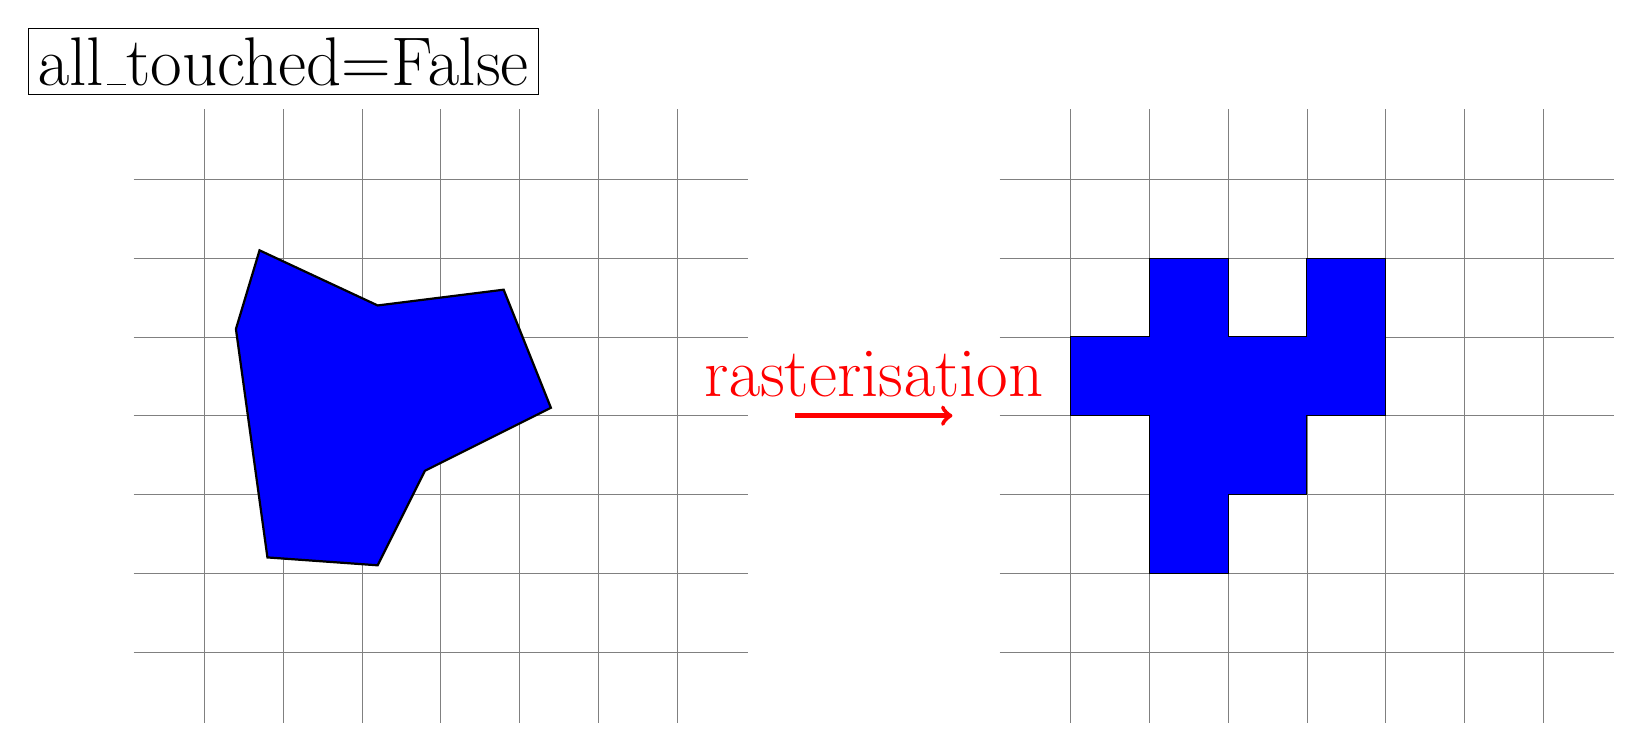
\begin{tikzpicture}
			\node[draw] at (0,6.5) {\Huge all\_touched=False};
			\draw[step=1cm,gray,very thin] (-1.9,-1.9) grid (5.9,5.9);
			\draw[fill=blue, thick] (-0.2, 0.2)--(-0.6, 3.1)--(-0.3,4.1)--(1.2,3.4)--(2.8,3.6)--(3.2, 2.6)--(3.4, 2.1)--(1.8,1.3)--(1.2, 0.1)--cycle;

			\draw[ultra thick,->, red] (6.5, 2) --node[above=1mm] {\Huge rasterisation} (8.5, 2);

			\draw[step=1cm,gray,very thin] (9.1,-1.9) grid (16.9,5.9);
			\draw[fill=blue] (11,0)--(11,2)--(10,2)--(10,3)--(11,3)--(11,4)--(12,4)--(12,3)--(13,3)--(13,4)--(14,4)--(14,2)--(13,2)--(13,1)--(12,1)--(12,0)--cycle;
		\end{tikzpicture}%
	}%
	\vspace*{5mm}
	\resizebox{8cm}{!}{
		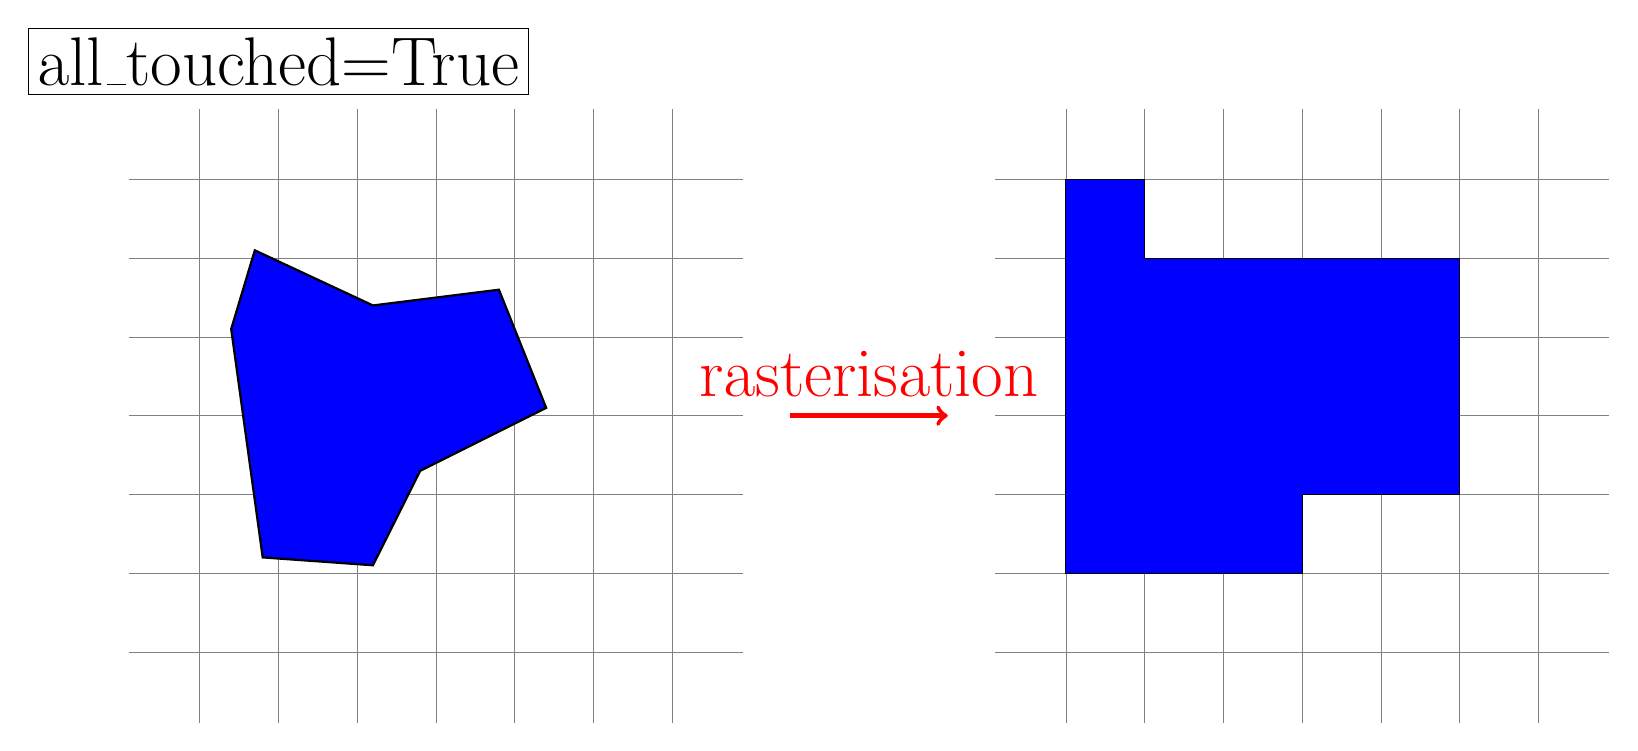
\begin{tikzpicture}
			\node[draw] at (0,6.5) {\Huge all\_touched=True};
			\draw[step=1cm,gray,very thin] (-1.9,-1.9) grid (5.9,5.9);
			\draw[fill=blue, thick] (-0.2, 0.2)--(-0.6, 3.1)--(-0.3,4.1)--(1.2,3.4)--(2.8,3.6)--(3.2, 2.6)--(3.4, 2.1)--(1.8,1.3)--(1.2, 0.1)--cycle;

			\draw[ultra thick,->, red] (6.5, 2) --node[above=1mm] {\Huge rasterisation} (8.5, 2);

			\draw[step=1cm,gray,very thin] (9.1,-1.9) grid (16.9,5.9);
			\draw[fill=blue] (10,0)--(10,5)--(11,5)--(11,4)--(15,4)--(15,1)--(13,1)--(13,0)--cycle;
		\end{tikzpicture}%
	}%
	\caption{Graphical example the rasterisation of a vector (left blue), to a raster (right blue) with either all~touched set to False (above), or True (below).}
	\label{fig:alltouched}

\end{figure}

\begin{table}[h!]
	\caption{Used levels of costs, the applied numerical equivalent and example layer this cost have been used for.}
	\label{tab:1}
	\centering
	\begin{tabular}{ l  r  l }
		Cost Level 			& Cost 					& Example\\
		\hline
		Prohibited 			& 500					& \makecell[lt]{Conversation areas as\\ National Parks, Buildings} \\
		Strongly Restricted & 10 					& \makecell[lt]{Conversation areas as Bird Reserve} \\
		Restricted 			& 5						& \makecell[lt]{Protected Landscape Area,\\ Industrial Areas, motorway, railway} \\
		No Restriction 		& 0.5					& Default\\
		Preferential 		& 0.1					& \makecell[lt]{Power Grid,\\ Motorway and Railway Buffers}\\
	\end{tabular}
\end{table}

The complete list of layers and the applied processing steps can be found in \textbf{Supplement S1}.

All three steps of the generation of the Least Cost Path: generation of the cost raster, aggregation and backtracking is shown with an example for a cost raster of 50~m resolution and all~touched set to False (see \ref{fig:costs2path}).

The chosen implementation applies early stopping.
Therefore, the costs for points that are not needed to try to connect to the end point are not aggregated (see figure \ref{fig:aggregation}).
After finding an aggregated cost for every end point, the aggregation stops and the backtracking starts.
Because the path ends at a power transformer, which is a building type, the paths end at in a \textit{Prohibited} area.
Therefore, areas even further away from the starting point have been explored first.

\begin{figure}
	\centering
	
	\subfloat[\centering Cost Raster.]{{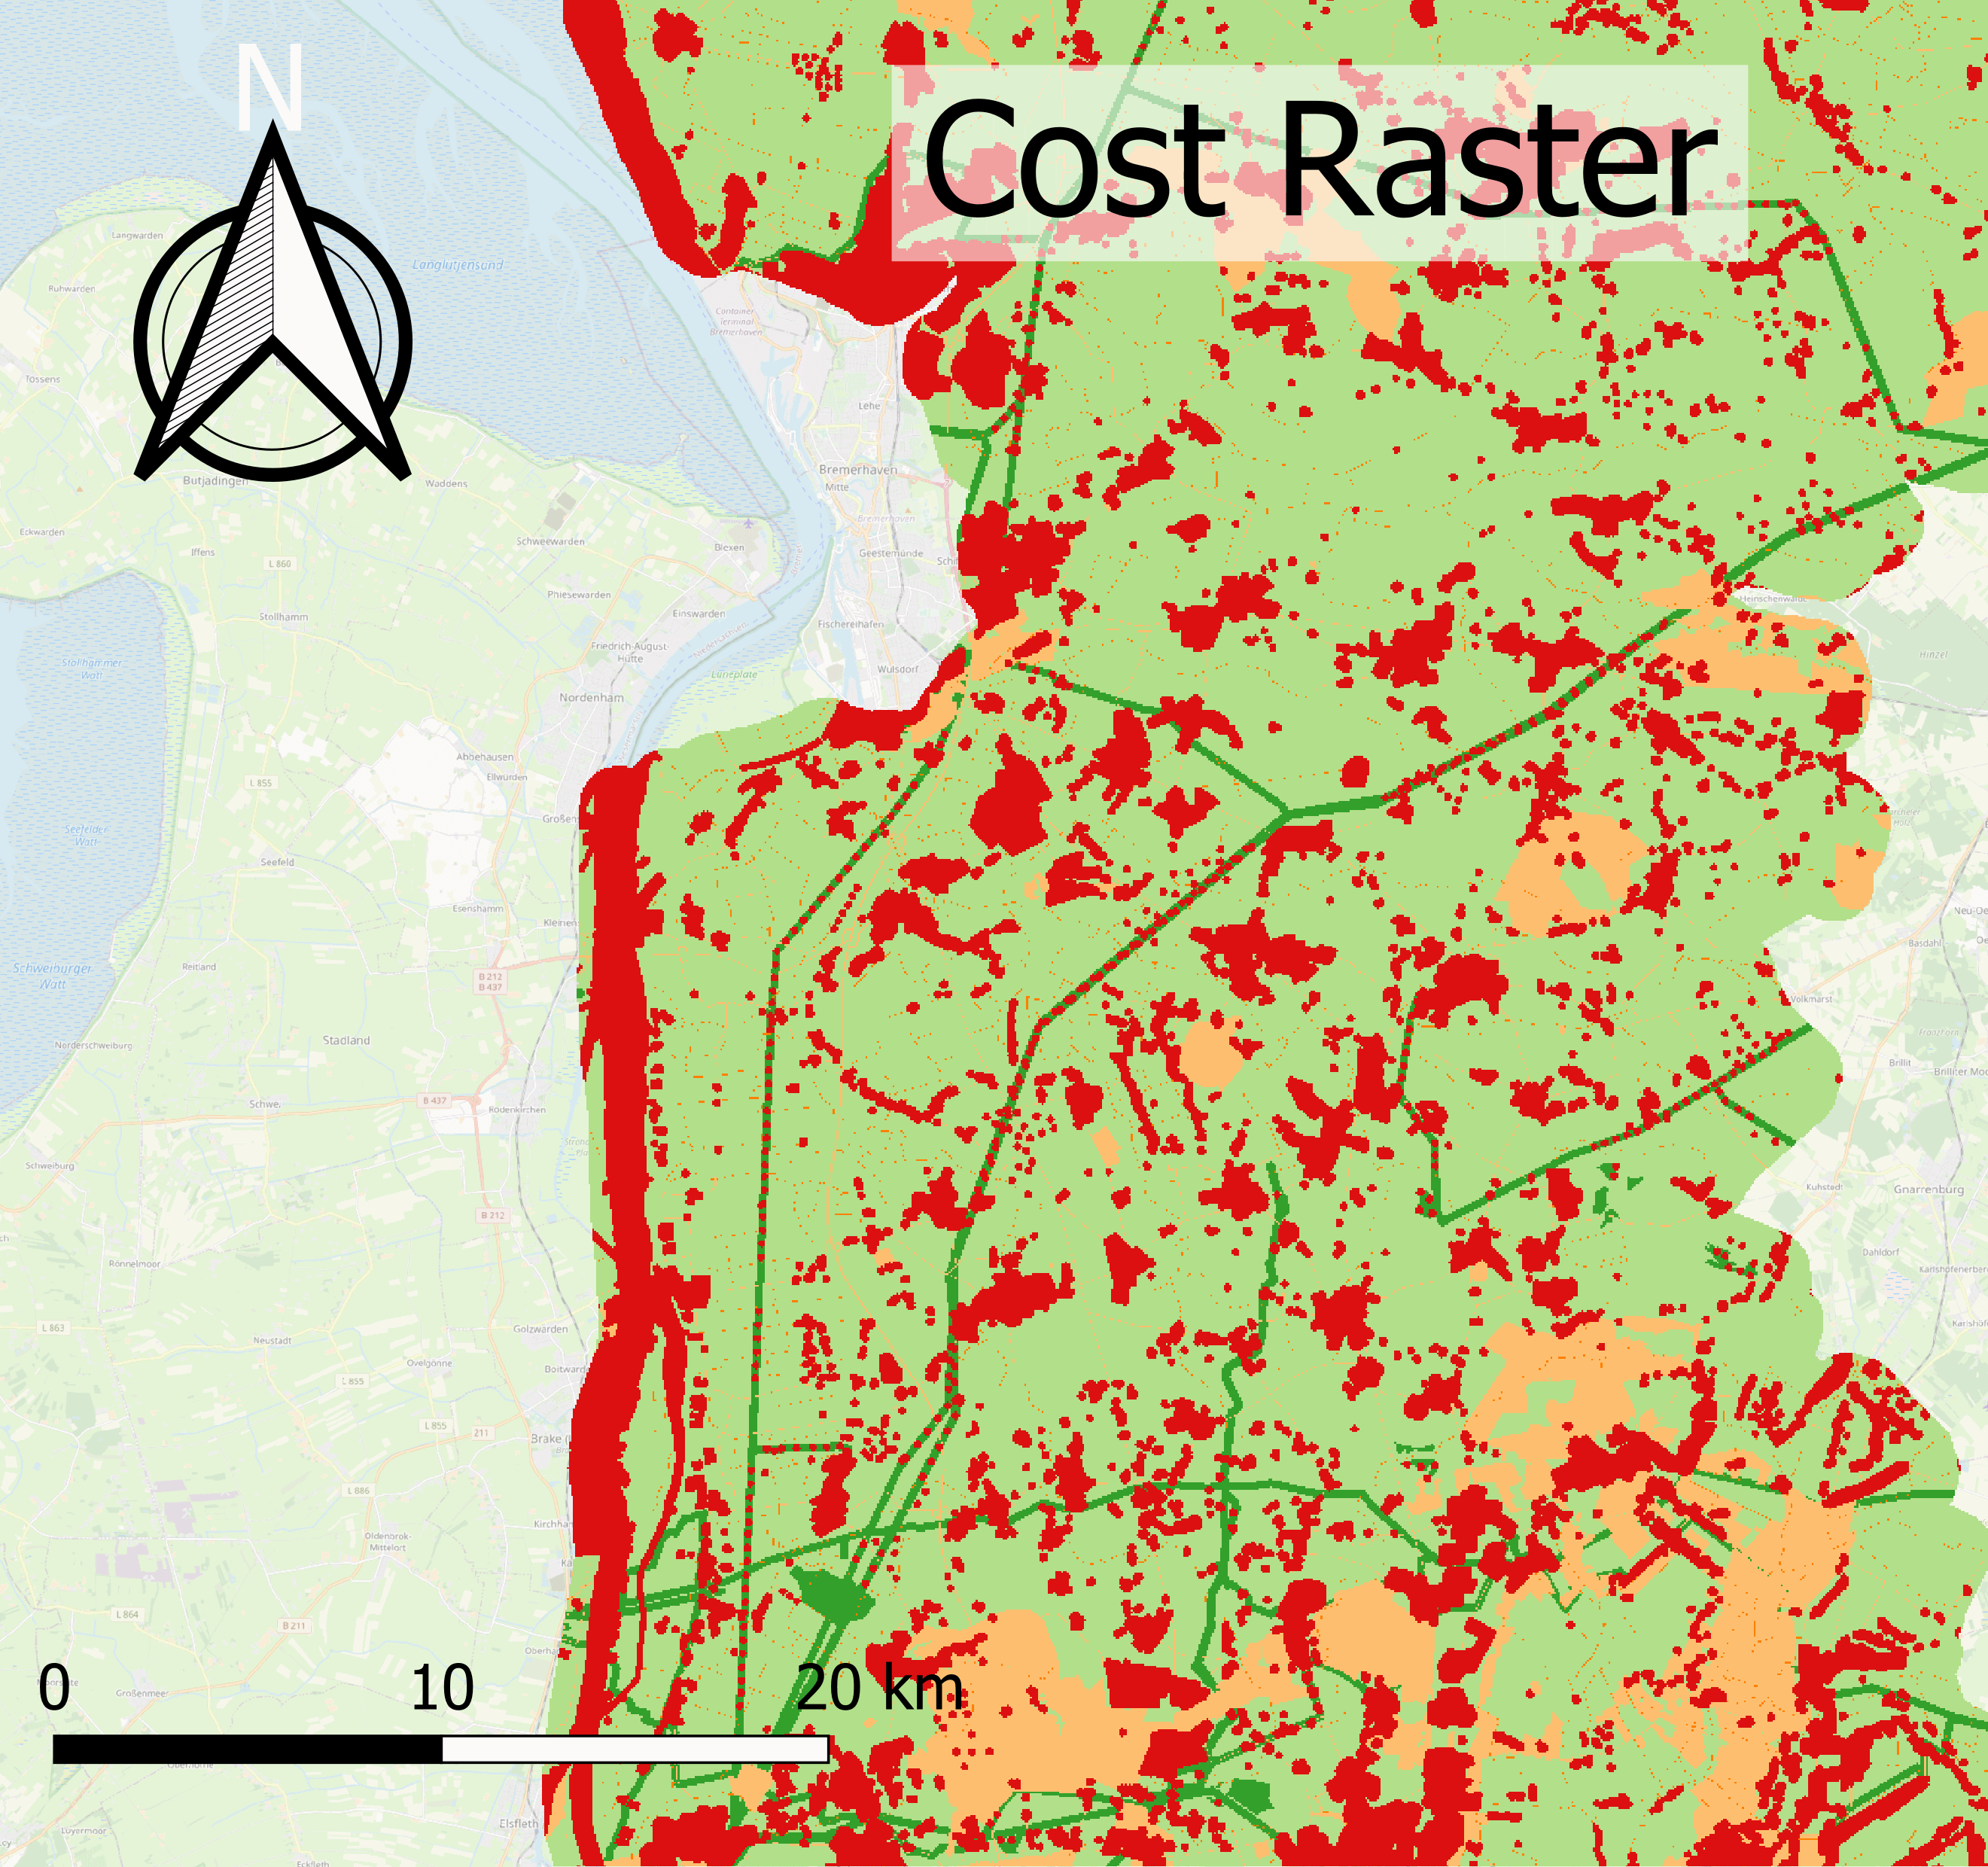
\includegraphics[width=.30\linewidth]{./images/CostRasterExample_cut.png} }}%
	\enskip
	\subfloat[\centering Aggregated Cost Raster.]{{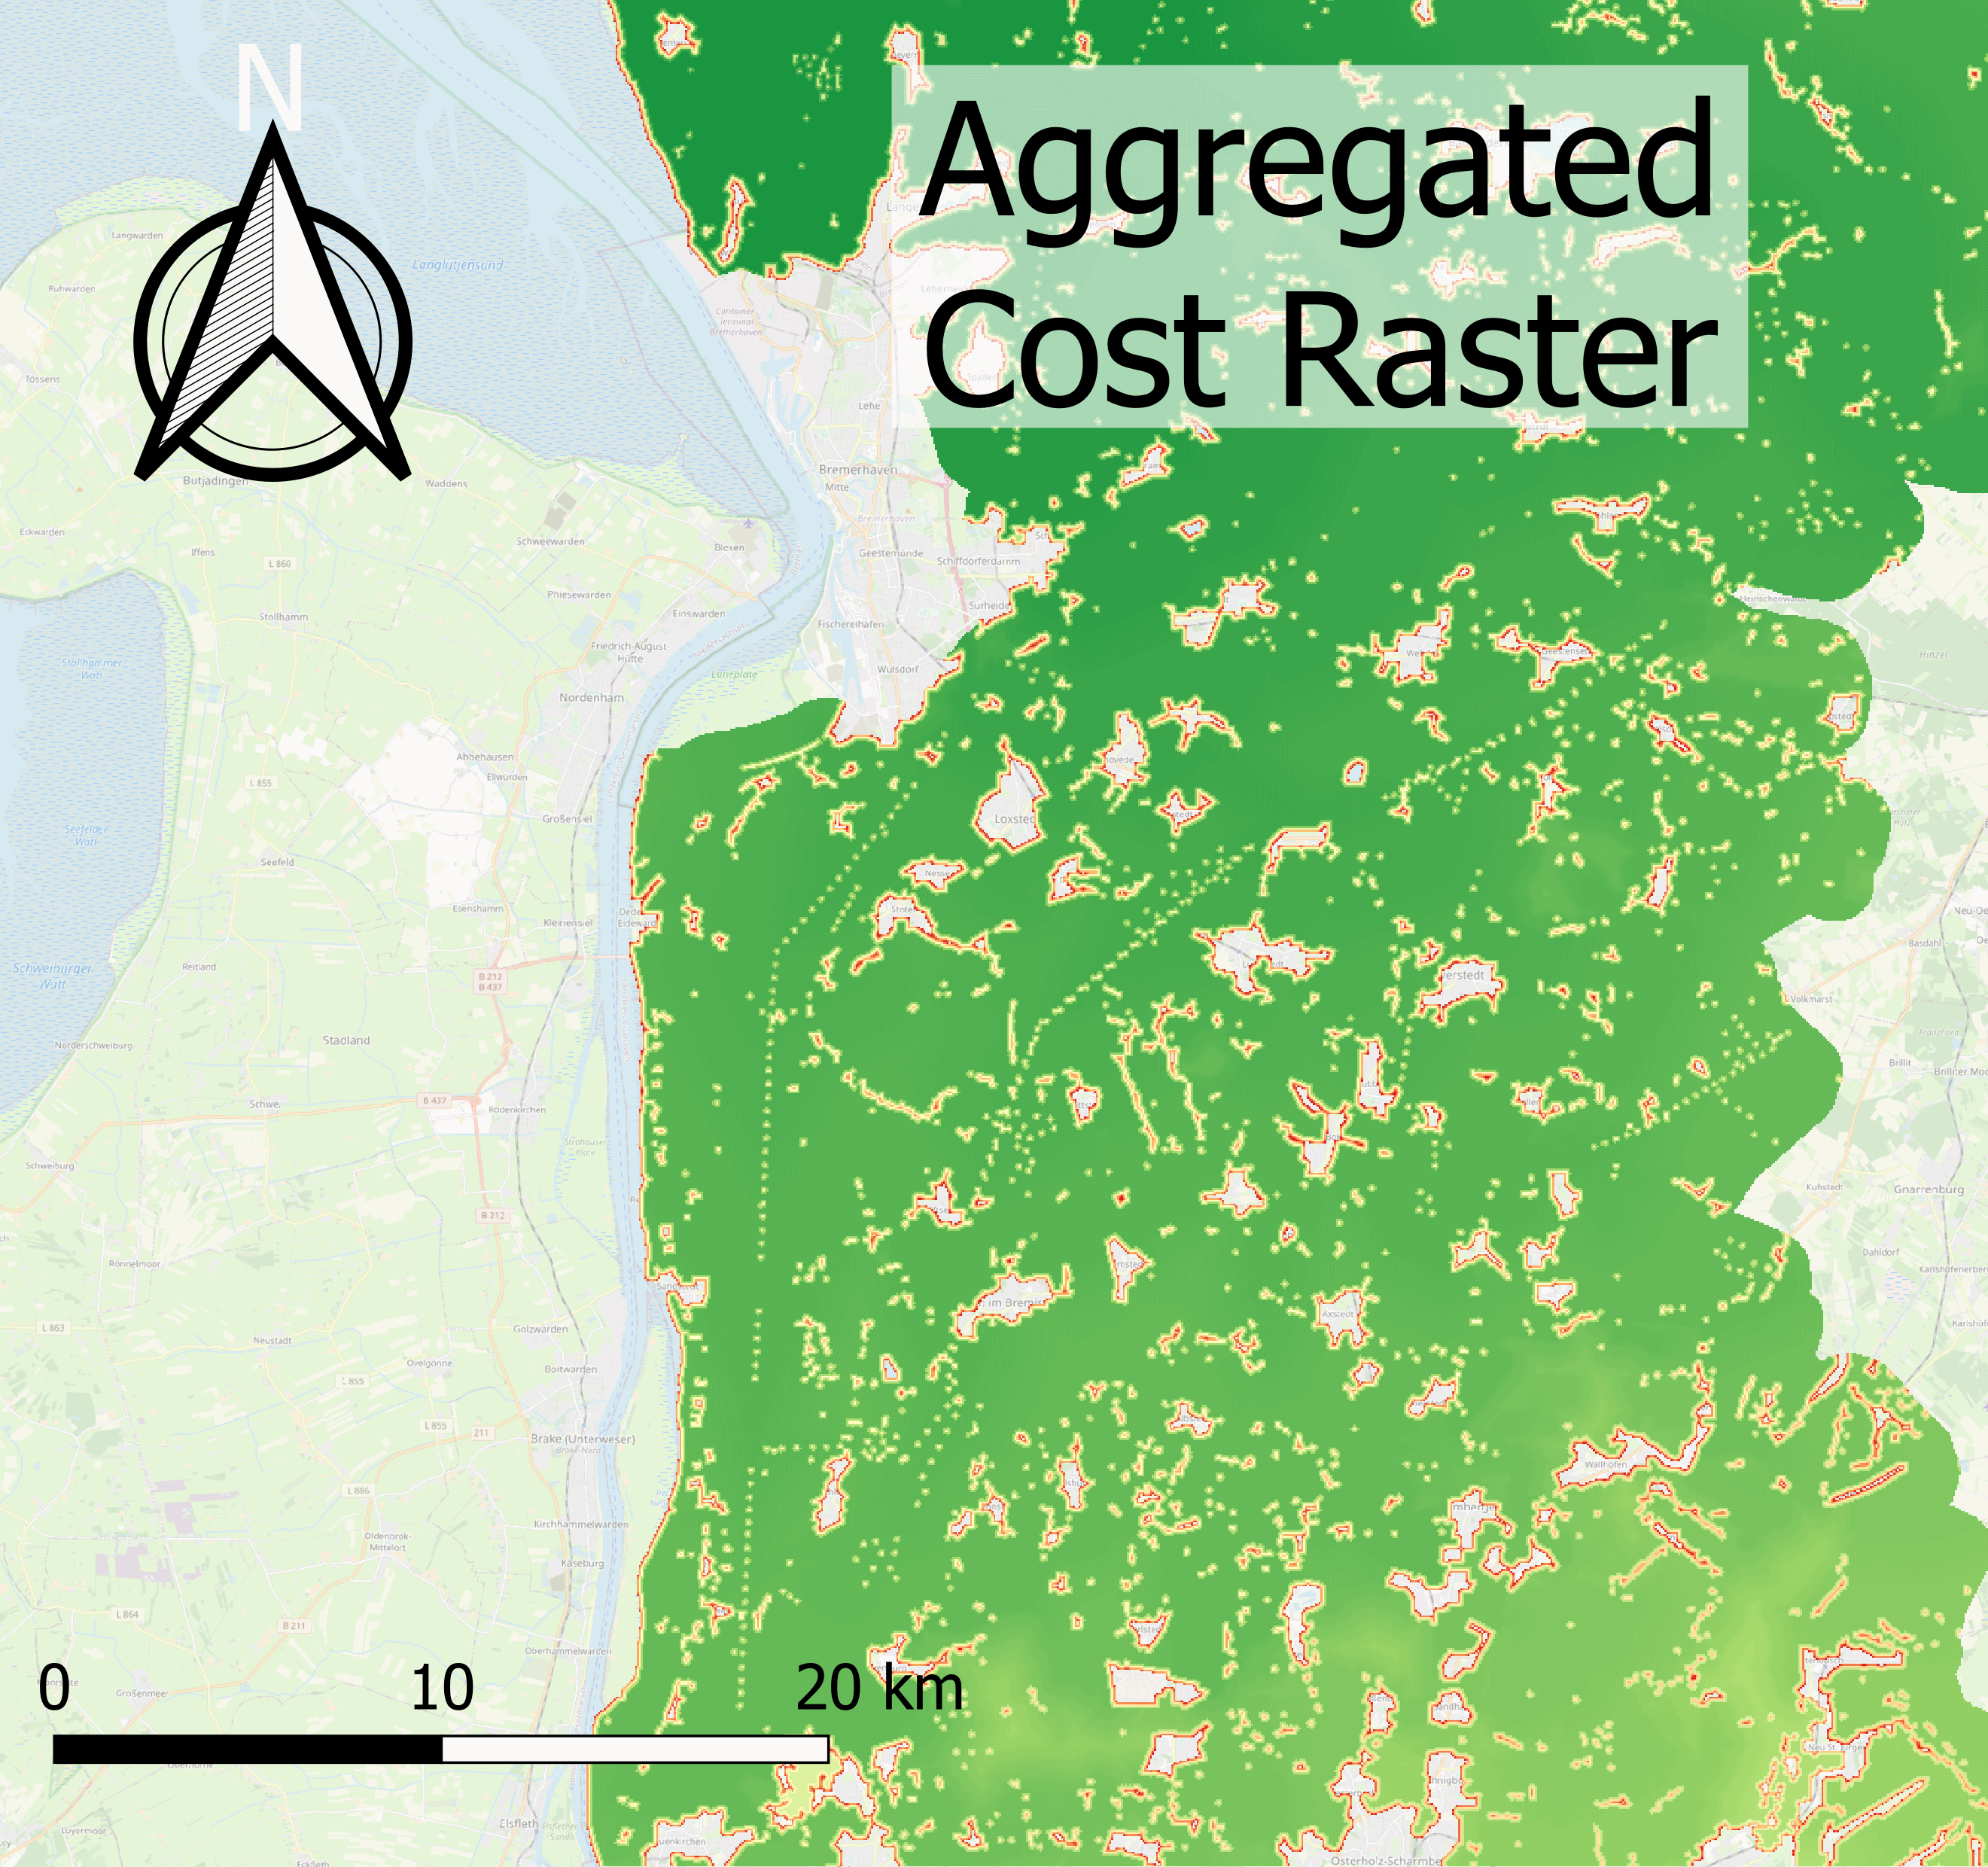
\includegraphics[width=.30\linewidth]{./images/AggregatedCosts_cut.png} \label{fig:aggregation}}}%
	\enskip
	\subfloat[\centering Least Cost Path.]{{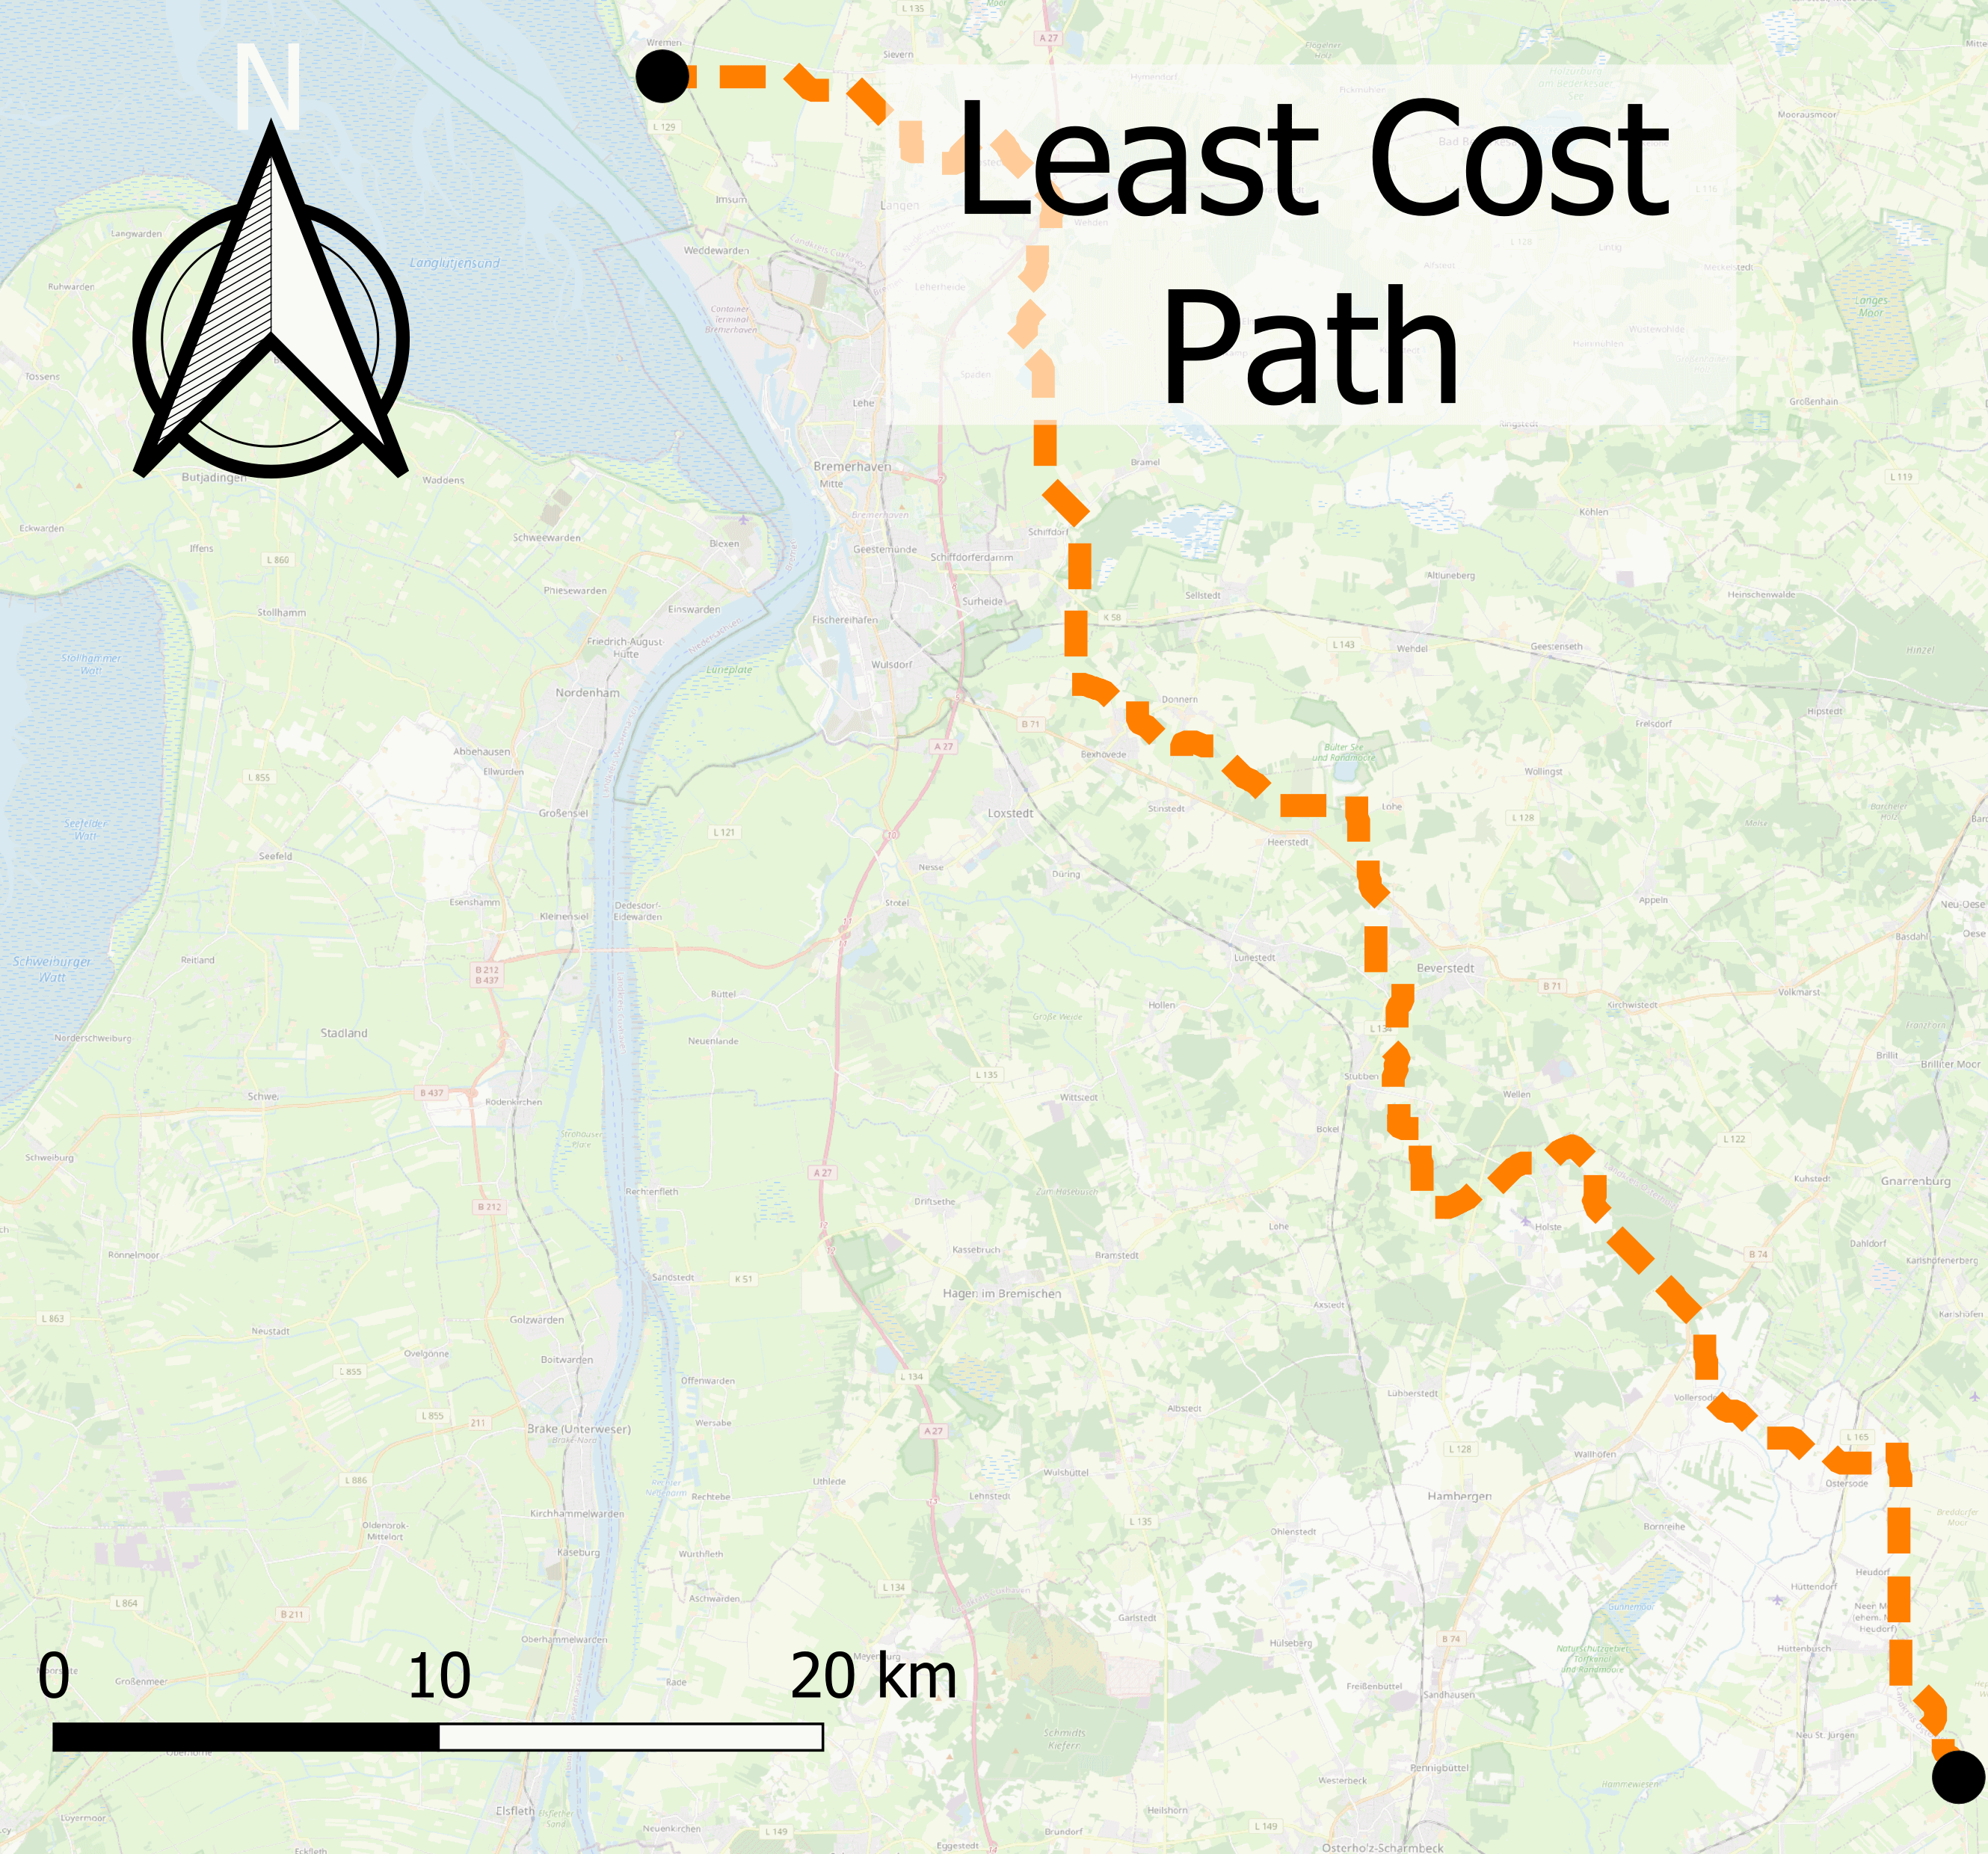
\includegraphics[width=.30\linewidth]{./images/LeastCostPathExample_cut.png} }}%

	\caption{Figures of the cost raster and the resulting aggregated costs and the Least Cost Path for a resolution of 50~m, all~touched set to False.}
	\label{fig:costs2path}
\end{figure}

	

%% Aggregation is implemented in a priority queue. 
%% Hence a point with a lower cost is evaluated earlier as a starting position to evaluate the cost of its neighbours, than a point with higher cost.


For low resolution rasterisation, with all~touched set to True will show every detail, but the objects are enlarged.
When all~touched is to False the object only appears, when the is situated at the pixel centre.
Thus, this might be used as surrogate, that expresses the likelihood of the object to be sampled and correlates with the object size  compared to the pixel size.
At high resolution the set all~touched to True still overestimates the object size, but the extent is limited.
Setting all~touched to False will include all objects for high resolution.
This setting is most realistic, because the over- and underestimation of the object size is limited to half a pixel size in every direction.
The best method should be to use the percentage of the pixel coverage by the object as weight, which is not possible.
As an alternative, switching between setting all~touched True and False may result in a better assessment of the true costs.
When superimposing the resulting cost raster, these map will include both aspects of the correctness: showing every detail and statistically distribute better the real cost.
Another method to achieve the same is to downsample high resolution raster.